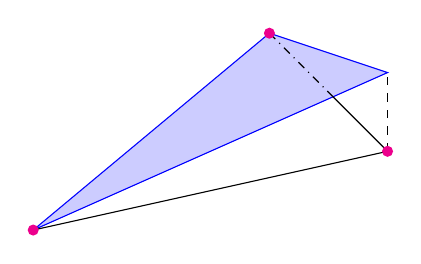
\begin{tikzpicture}	
	\coordinate (A) at (0,0);
	\coordinate (B) at (3,2.5);
	\coordinate (C) at (4.5,1); % pivot	

	\coordinate (T) at (4.5,2);
	
	\draw[dashed] (C)--(T);
	\fill[blue!20] (A)--(B)--(T)--(A);
	\draw[blue] (A)--(B)--(T)--(A);
	
	\draw (A)--(C)--(3.8,1.7);
	\draw[dash dot] (B)--(3.8,1.7);
	
	\foreach \p in {(A),(B),(C)}	
		\fill[magenta] \p circle (2pt);
\end{tikzpicture}